%\documentclass[subscriptcorrection,upint,varvw,barcolor=BrickRed,
%mathalfa=cal=euler,balance,hyphenate,pdf-a,nocopyright]{asmejour} 

\documentclass[barcolor=BrickRed,nocopyright,nolists]{asmejour} 
%\usepackage[usenames,dvipsnames]{xcolor}
\usepackage{tikz} 
\usepackage{tikz-layers} 
\usepackage{physics}
\usetikzlibrary{calc, arrows.meta, intersections, patterns, positioning, shapes.misc, fadings, through,decorations.pathreplacing}
\usetikzlibrary{positioning,shapes,arrows,backgrounds,external,fit,calc}
\usetikzlibrary{shapes.geometric,shapes.arrows,fit,positioning}
\usetikzlibrary{3d, arrows.meta, bending, calc, perspective}
\usetikzlibrary{perspective}
\usetikzlibrary{patterns,decorations.pathmorphing}
\usetikzlibrary{decorations.markings}
\usetikzlibrary{arrows.meta}
\usetikzlibrary{calc}
\tikzset{>=latex}
\usepackage{array}
\usepackage{pdfpages}

%%%%  pdf metadata  %%%%

\hypersetup{
	pdfauthor={Ahmad Assadeq},                       		   	
	pdftitle={Koval Factor For A Five-Spot Pattern Using Reservoir Simulation}, 
	pdfsubject = {Koval Factor For A Five-Spot Pattern Using Reservoir Simulation},
}

%\JourName{Ms Report}
\PreprintString{PGE388 Advanced Reservoir Engineering Project}[R]
\PreprintString{}[L]

\begin{document}

\SetAuthorBlock{Ahmad Assadeq}{The University of Texas at Austin,\\
   Hildebrand Department of Petroleum and Geosystems Engineering (UT PGE),\\
   Austin, Texas, USA\\
   aoa442@my.utexas.edu} 

\title{Koval Factor For A Five-Spot Pattern Using Reservoir Simulation}

\keywords{Reservoir Engineering, Koval Factor, Waterflooding, Immiscible Displacement.}
   
\begin{abstract}
	The Koval method was invented in 1963 to tackle the issue of viscous fingering and early breakthrough
	of solvent injected in the reservoir. However, the method can be extended to immiscible flood if the 
	segregated flow condition is satisfied. 
	The \textit{MATLAB Reservoir Simulation Toolbox} is used to simulate a Homogeneous Quarter Five-Spot 
	to find the best fit for .
\end{abstract}
							
\maketitle %% This command creates the author/title/abstract block. Essential!

%%%%%%%%%%%%%%%%%%%%%%%%%%%%%%%%%%%%%%%%%%%%%%%%%%%%%%%%%%%%%%%%%%%%%%%%%%%%%%%%%%%%%%%%%%%%%%%%%%%%%%%

\section{Introduction}
The prediction of oil production is related to the multiphase fluid flow in porous media. This physical phenomena
is complicated due to the nonlinearity of the problem. Fluid dynamics of the flow is affected by the viscosity
and density ratios of the fluids present, relative permeability and capillary pressure also introduce additional challenges.
In the case of a displacing fluid having higher relative permeability it will move rapidly into the resident fluid and produce
shock fronts and rarefaction waves. These would result in early breakthrough for homogenous reservoirs and viscous fingering in 
hetrogeneous ones. \textit{Viscous fingering} is the unevenly displacement of one fluid by another. 

\subsection{Areal Sweep Efficiency}

\begin{figure}[h]
	\centering\scalebox{1}{\colorlet{mydarkblue}{blue!40!black}
\colorlet{myblue}{blue!70!black}
\colorlet{myred}{red!65!black}
\colorlet{myorange}{orange!90!black!90}
\colorlet{vcol}{blue!45!black}
\colorlet{watercol}{blue!80!cyan!10!white}
\colorlet{darkwatercol}{blue!80!cyan!80!black!30!white}
\colorlet{metalcol}{blue!25!black!30!white}
\tikzstyle{piston}=[blue!50!black,top color=blue!30,bottom color=blue!50,middle color=blue!20,shading angle=0]
\tikzstyle{water}=[draw=mydarkblue,rounded corners=0.1,top color=watercol!90,bottom color=watercol!90!black,middle color=watercol!50,shading angle=20]
\tikzstyle{horizontal water}=[water,top color=watercol!90!black!90,bottom color=watercol!90!black!90,middle color=watercol!80,shading angle=0]
\tikzstyle{metal}=[draw=metalcol!10!black,rounded corners=0.1,top color=metalcol,bottom color=metalcol!80!black,shading angle=10]
\tikzstyle{vvec}=[->,very thick,vcol,line cap=round]
\tikzstyle{force}=[->,myred,very thick,line cap=round]
\tikzstyle{width}=[{Latex[length=4,width=3]}-{Latex[length=4,width=3]}]
\def\tick#1#2{\draw[thick] (#1)++(#2:0.12) --++ (#2-180:0.24)}

\begin{tikzpicture}[x={(1cm,0)},y={(0.55cm,0.40cm)},z={(0,1cm)}]
  \def\L{1.8}   % cube side
  \def\H{1.2}   % total height
  \def\d{0.8}   % total distance
  \def\N{7}     % number of layers
  \def\t{\H/\N} % layer thickness
  \def\layer#1#2#3#4{
    \draw[#1] (#2+\L,0,#3) --++ (0,\L,0) --++ (0,0,-#4) --++ (0,-\L,0) -- cycle;
    \draw[#1] (#2,0,#3) --++ (\L,0,0) --++ (0,0,-#4) --++ (-\L,0,0) -- cycle;
    \draw[#1] (#2,0,#3) --++ (\L,0,0) --++ (0,\L,0) --++ (-\L,0,0) -- cycle;
  }

  \layer{metal}{0}{0}{0.6*\t}
  \foreach \i [evaluate={\x=(\i-1)*\d/(\N-1); \ya=\i*\H/\N; \yb=(\i-1)*\H/\N;}] in {1,...,\N}{
    \layer{water}{\x}{\ya}{\t}
  }
  \layer{metal}{\d}{\H+0.6*\t}{0.6*\t}
  \draw[vvec] (1.4*\L+\d,\L,\H-0.5*\t) --++ (1,0,0) node[below=0,right=-1] {$f$};
	\node at (\d-0.45*\L,0.2*\L,\H+0.6*\t) {$N$};
\end{tikzpicture}
}
	\caption{Heterogeneous layered reservoir.}
	\label{heterogeneous}
\end{figure}

\begin{equation}
	F = \frac{\sum_{i=1}^{n}k_{i}h_{i}}{\sum_{i=1}^{N}k_{i}h_{i}}
\end{equation}

\begin{equation}
	C = \frac{\sum_{i=1}^{n}\phi_{i}h_{i}}{\sum_{i=1}^{N}\phi_{i}h_{i}}
\end{equation}

\begin{itemize}
	\item [$F$] Flow capacity.
	\item [$C$] Storage capacity.
	\item [$N$] Total number of layers in the reservoir.
	\item [$n$] A number between $1$ and $N$.
\end{itemize}

\begin{equation}
	F = \frac{1}{1 + \frac{(1-C)}{H_{K}C}}
\end{equation}

\subsection{Koval Modifiction For Heterogenous Systems}
Koval theory is used to predict solvent cut and oil recovery in a miscible displacement as a function of the pore volumes of solvent injected into a core \cite{salazar}.
The Koval method describes heterogeneity by a factor $K_{V}$, the $K_{V}$ is a product of the heterogeneity effects  $H_{K}$ and 
an effective mobility ratio $E$. Koval's method is a simple estimation of oil recovery and solvent in a miscible displacement as a
function of the pore volumes of solvent injected into a core. If the flow is segregated between the displacing and resident fluid
the Koval method can also be applied for any kind of displacement.

\subsection{Advantages Of Simulating Areal Sweep Problems}
The combination of physical effects on areal sweep is not very clear. Gravity segregation can force fluids with different density
to segregate. Capillary forces tend to spread out the interface between different fluids. Adding heterogeneity makes the prediction 
fluid movement in the reservoir very complicated without using numerical simulation. In some cases, the different forces can combine to 
reduce the sweep and displacement efficiency, and in others they can reduce the fingering and delay the breaktrhough.

%%%%%%%%%%%%%%%%%%%%%%%%%%%%%%%%%%%%%%%%%%%%%%%%%%%%%%%%%%%%%%%%%%%%%%
\section{MRST Simulation Of Quarter-Five Spot}
To investigate the problem of finding the best Koval-Factor for a Five-spot pattern with uniform permeability, 
the \textit{MATLAB Reserservoir Simulation Toolbox} (\texttt{MRST}) will be used for simulation. This collection
of \texttt{MATLAB} modules and code snippets for simulation different typical reservoir engineering problems is 
a good starting point for research on reservoir simulation projects. The library already has code snippets for
simulating a \textit{Homogeneous Quarter Five-Spot}\cite{mrst}.
\begin{figure}[h]
	\centering\scalebox{0.8}{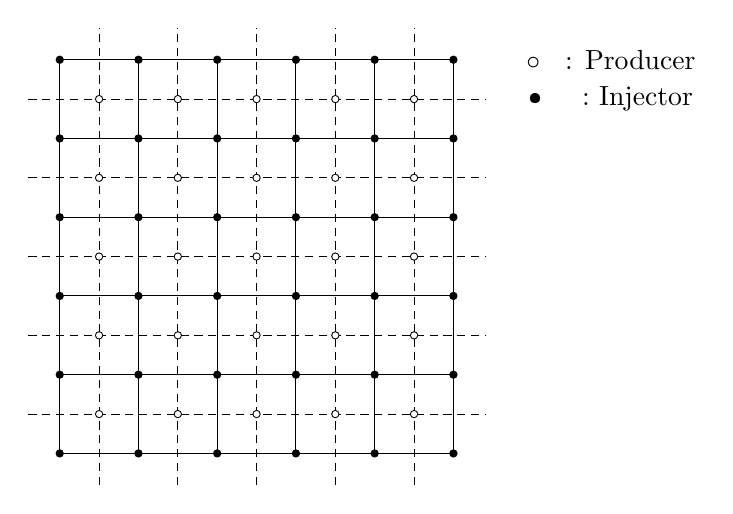
\begin{tikzpicture}
\draw (0,0) grid (5,5);
\draw[densely dashed, shift={(-.5,-.5)}] (.1,.1) grid (5.9,5.9);
\draw[line width=3pt, line cap=round, dash pattern=on 0pt off 1cm](0,0) grid (5,5);
\draw[shift={(-.5,-.5)}, double, double distance=2.2pt, line cap=round, dash pattern=on 0pt off 1cm] (1,1) grid (5,5);
	\node at (7,5) {$\circ$ \hspace{0.2cm}: Producer};
	\node at (7,4.5) {\textbullet \hspace{0.5cm}: Injector};
\end{tikzpicture}
}
	\caption{A repeated five-spot pattern.}
	\label{fivespot}
\end{figure}
The \textit{repeated five-spot pattern}, which consists of a thin, infinitely large, horizontal reservoir with a staggered
pattern of injection and production wells as \ref{fivespot} that repeats itself to infinity in all directions. By fixing the 
rates for all wells the flow pattern has certain symmetries and its common to consider one tile subject to no-flow boundary
conditions.

A single phase quarter five-spot can be formulated as solving $-\nabla \cdot (\mathbf{\vec{K}}\nabla p) = q$ with no-flow boundary
conditions and two source terms at diagonally opposite corners of a 2D Cartesian grid covering a $500\times500$ $m^{2}$ area.
The rectangular grid has homogeneous petrophysical properties ($K= 100$ mD and $\phi = 0.2$). The purpose of this example is to:

\begin{enumerate}
	\item In addition to computing pressure, we will also compute streamlines from
	\item the flux field as well as the corresponding time-of-flight, i.e., the
	\item time it takes for a neutral particle to travel from a fluid inlet (source
	\item term, well, inflow boundary, etc) to a given point in the reservoir.
\end{enumerate}

The discretization and solution in this example uses the simple \textit{Two-Point Flux Approximation} (TPFA).


\subsection{MIMD On The Heterogeneous Element Processor}
In their 1987 study of parallel reservoir simulation, Scott, et al.\cite{spe16020} presented the parallelization of two time consuming tasks in reservoir simulation: Jacobian construction and linear solver.
Their study was conducted on two parallel machines the \texttt{Heterogeneous Element Processor} computer produced by Denelcor and the Intel \texttt{iPSC Hypercube}. One intention of this paper was to show
the potential of MIMD machines for reservoir simulation. The Jacobian construction for both black-oil and compositional types were presented and both direct and iterative linear solver methods were addressed 
for parallelization. In forming the Jacobian matrix, the authors mention that when the simulator is performing table-lookup for PVT or saturation tables the operation can be divided among processors and performed
in parallel. In compositional simulation, the phase equilibrium and fluid property calculations are amenable to parallelization.

\subsection{Buckley-Leverett Problem On The \texttt{CM}}
The work of Mayer\cite{spe19121}, discussed the parallelization of the explicit formulation of the Buckley-Leverett problem on the \texttt{Connection Machine}. The paper discussed the possibilities of different strategies
of distribution of gridblocks among the processors. From centralized storage of relative permeability curves on a single node to possible distributions of well data among nodes. Communication among nodes is minimized by excluding processors holding information
for inactive gridblocks. In this study, the largest size of the model used was over $8$ millions gridblock. The \texttt{Connection Machine} has $65 \ 636$ processors.

\subsection{Wheeler and Smith \texttt{Hypercube}}
One of the first attempts to design a reservoir simulator that utilizes the parallel programming paradigm was the research project carried by Wheeler and Smith\cite{spe19804}.
The simulator was an implicit, 3-D, two phase (oil, water), and ran on the \texttt{Intel iPSC/2 Hypercube} supercomputer. This \texttt{Intel} machine is referred to as a cube since 
the topological configuration of the computing nodes are similar to that of a cube, that is each computing node resides on the corner of the cube and cube edges are considered the 
communication lines. The interprocess communication was performed using \texttt{FORTRAN} calls. The programming concepts that are needed to program such
a simulator are related to computational grid partitioning and inter processor communications. The simulated reservoir model must be partitioned among the computing cores
of the 16-node machine, and then the code for the different components of the simulator must be designed in a way that minimizes the communication between the processors.
Communication is, of course, necessary between adjacent domains to send and receive boundary variables along shared gridblocks.
The research work of Wheeler and Smith focused on implementing different parts of the simulator to run efficiently on parallel. Their research paper included a discussion of
the linear solver, that was implement specifically for the parallel machine. The distribution of gridblocks among the processors is done vertically, that is each griblock along a vertical line
through the computational domain is given entirely to a processor (Z-lines distribution strategy), see figure (\ref{cube}).

As in the vector processing machines introduced early, a knowledge of the computing machine architecture is also required to efficiently program the \texttt{Hpyercube} computer\cite{duchark}.
However, the \texttt{Hypercube} computer started the revolution of developing reservoir simulators for distributed-memory machines. This enabled the run of larger model sizes and the spreading
of code parallelization concepts that will prove essential later when programming high performance computers will become more and more architecture independent.

\subsection{Parallel Compositional Reservoir Simulation}
The work of Wheeler and Smith focused on black-oil type fluid models. Compositional fluid models were the focus area of John Killough and Rao Bhogeswara\cite{spe21208}. They based their studies on
three reservoir models, an enlarged version of \textit{Third SPE Comparative Solution} problem, a highly hetrogenous problem and a hypothetical model. One important feature of the computing machine used in this study, the \texttt{iPSC/860}, is that no knowledge of the
machine architecture and topology was required to program it. The study investigated the parallelization of the commercial simulator \textit{VIP-COMP} from Western Atlas Integrated Technologies. Only the IMPES option of the simulator was parallelized for the study. 
The authors initially profiled the simulator and targeted most time consuming parts of the simulator. Jacobian construction and the linear solver were the most time consuming parts of the simulator. 
The flash computations (PVT computations for the compositional fluid) were also time consuming. The coefficient matrix setup was reported to achieve excellent parallelization. The parallelization of data structures of the simulator was also necessary.
The use of \texttt{Asynchronous} (nonblocking) message passing was also used in developing the simulator.

\subsection{IMPES Compositional Simulator On \texttt{CM-2}}
Published in 1992, Rutledge, et al., described an IMPES formulation with seven-point stencil discretization scheme simulator. The focus of the work was on techniques suitable for a SIMD machine. The simulator was designed to run on \texttt{Connection Machine-2}.
The \texttt{CM-2} is a . The linear solver used in this simulator was the Generalized Minimum Residual iterative solver \texttt{GMRES}. The data structure used in this simulator partition the gridblocks including inactive ones to all processors. This may risk some
processors to be (all-inactive gridblocks owner) that is an idle processor. The issue of replicating PVT and saturation table lookups is discussed. The solution undertaken in the study uses a feature of the \texttt{CM-2} machine. The tables are distributed among
nearby groups of processors, this enables each processor in a 32-processor cluster to gather and assemble the table efficiently. This is possible by turning the table lookups to single point arithmetic precision, which is sufficient for table lookups of physical properties.
In this study well terms were all treated on a single processor (the front end), as opposed to distributing wells among processors. The \texttt{CM-2} machine was invented before the MPI standard, therefore, the machine specific communication routines were used. These were the
\texttt{NEWS} and \texttt{SEND} data communication routines, the first for nearest neighboring processor the second for communication between any two processors in the cluster. The use of the \texttt{SEND} was minimized to increase the performance of the simulator. However, the
linear solver required the use of \texttt{SEND} routine.

\subsection{Parallelization Of LGR And AIMP}
This work discussed the paralellization of \textit{Local Grid Refinement} and \textit{Adaptive Implicit Schemes} in reservoir simulation. Both of these two features are employed in studying field models and cases where the application of fully-implicit fully refined reservoir models
with limited computer resources is difficult. The fast-changing dynamic parts of the reservoir model, for example, near-wellbore regions, high permeability with fast flow regions and solvent fronts are refined or treated in a fully-implicit fashion. While, the other slowly varying regions
of the reservoir are coarsened and treated explicitly. These two features raise an additional challenge to parallelization, since now computational demands vary from region to another in the reservoir. In their implementation of the Jacobian construction, cells are grouped according to their
implicitness and only active cells are included. Vectorization of the inner loops in property calculations was also performed to gain an increase of performance. A further classification of gridblocks according to their fluid phase is also performed. For an illustration of Local Grid Refinement,
see figure (\ref{lgr}).
\begin{figure}[h]
	%\centering\scalebox{0.5}{\input{lgr.tikz}}
	\caption{Local Grid Refinement Illustration.}
	\label{lgr}
\end{figure}

\subsection{Statoil Parallel Reservoir Simulator On \texttt{MasPar MP-2}}
This simulator is black-oil, two-phase, sequential implicit. It ran on a SIMD, $16 \ 384$ processors machine, named \texttt{MasPar MP-2}. It used Krylov subspace methods for linear solution of the system of equations. The pressure system is solved using a two level Additive Schwarz preconditioner. Other linear solution
methods are also implemented in the simulator for coarse grid regions to enhance efficiency. The research pays attention to problems of numerical dispersion produced by the use of finite-difference discretization and upstream weighting. The general rules of thump principles were followed to design this parallel siimulator:
data locality, domain decomposition, minimized communications and boundary data duplication between neighboring processors. The discretization method used in this simulator is the finite-element (Galerkin formulation). The Krylov space method used for the linear system is the Conjugate Gradients method. The saturation system
is solved using a hyperbolic solver, that used the Modified Method Of Characteristics, this solver was inefficient when compared to the pressure solver. It consumed 4 times more than the pressure system. 

\subsection{Amoco Falcon Parallel Reservoir Simulator}
In 1998, Amoco published results regarding their simulator made in cooperation with Los Almos National Laboratory and Cray Research\cite{spe51969}. They report increased efficiency of run time as high as $100$ faster than previous vector machines. The simulator was written in \texttt{FORTRAN90} and follows the SIMD programming paradigm.
The simulator was tested on multiple parallel platforms including \texttt{CRAY T3D}, \texttt{SGI Power Challenge}, \texttt{Origin 2000}, \texttt{CM-5} and \texttt{IBM SP2}. The linear solver is implemented as an incomplete lower-upper (ILU) preconditioner coupled with \texttt{GMRES} or \texttt{ORTHOMIN} as iterators.
The authors report the ability of the simulator to run large (up to $16.5$ million gridblocks) scale simulations. The simulator uses the High Performance Fortran Extension (HPF) for communication among processors, in contrast to MPI. The simulator implements an Adaptive Implicit approach to mobility. Mobility can be treated explicitly,
but this may increase the risk of instability of the simulation run. The simulator is compositional with two linear solver packages. The linear solver package is selected based on the type of simulation: Red/Black Z-line Successive Overlaxation (\texttt{SOR}) for IMPES and a Krylov \texttt{GMRES} or \texttt{ORTHOMIN} with \texttt{ILU} preconditioner for fully implicit.

\subsection{Aramco First Reservoir Simulator \texttt{POWERS}}
The salient feature of the in-house developed, \textit{Parallel Oil Water Enhanced Reservoir Simulator}\cite{spe75805} of Saudi Aramco is its robust ability to handle the some of the largest reservoir models in the industry. This requirement is expected since reservoirs sizes in Saudi Arabia are usually larger than reservoirs from other parts of the world. The engineers in Saudi Arabia
started their work in reservoir simulation development by improving the performance of \textit{MARS} reservoir simulator developed by Exxon Production Research Company\cite{spe11483}. Their work on the \textit{MARS} simulator was mainly done on increasing vectorization and parallelization of the linear solver\cite{spe29856}. In 1996, Saudi Aramco deployed the $POWERS$
simulator. It is typical for small and medium size reservoirs to have grid size of $50 / m$, however Middle East reservoirs with grid size of $250 / m$ produce models with $1$ million cells. Therefore, the aim of \texttt{POWERS} was to be able to handle megacell simulations with ease. The simulator is a three dimensional, three-phase, with generalized compositional
formulation (black-oil is a specialized case) with the ability to define multiple PVT and saturation tables for different regions, that is it supports multiple equilibration regions. Two discretization methods are implemented: IMPES and the fully-implicit method. All of the main components of the simulator: Jacobian construction, linear solver, property calculations 
are written in parallel. The simulator was ran on several High Performance Computing platforms: \texttt{CM-5, IBM-NH2, SGI Origin 3800}. The linear solver options of the simulator are generalized conjugate residual and Orthomin with truncated Neumann series as a preconditoiner. The simulator also featured: a Local Grid Refinement, a Well Management package, Integration to 
Pre- and Post-processing software. The simulator is reported to reduce simulation time of giant reservoirs from days to hours.

\subsection{Aramco Second Reservoir Simulator \texttt{GigaPOWERS}}
The second generation Aramco simulator extended the capability of the previous one. It manages to run large model sizes of up to a bilion cells. It also provides a collection of features that were not available in the previous simulator. The new simulator was named \texttt{GigaPOWERS}, the same previous name prefixed with \texttt{Giga}, to indicate its 
ability to run ($10^{9}$) cells. The simulator was deployed in 2009\cite{spe119272}. The new features added to the simulators include: a Distributed Unstructured Grid Infrastructure (enhanced parallel capability to handle unstructured grids), Complex Well Modeling (Multi-lateral wells with Inflow Control Vales and Devices), Dual-Porosity Dual-Permeability
(to handle faults in a reservoir) and an improved linear solver that handles systems of equations resulting from unstructured grids more efficiently. The formulation used in the simulator is the generalized compositional formulation used previously in \texttt{POWERS}. The \texttt{GigaPOWERS} simulator also performs the reading and writing of input and output
(IO) files in parallel. The simulator also supports the standard Corner Point Geometry (CPG): non-orthogonal structured grid used typically in reservoir simualtion, see figure (\ref{cpg}). Another important additon to the \texttt{GigaPOWERS} simulator is the development of an Optimizatoin Based Well Management. This enables the advanced treatment and handling of reservoir engineering
production strategies, by solving a minimization problem internally. The simulator ran on different hardware environments: clusters with \texttt{Intel Xeon} and \texttt{AMD} processors, along with \texttt{IBM BlueGene/P} and \texttt{SGI Altix}.
\begin{figure}[h]
	%\includegraphics[scale=0.12]{cpg.pdf}
	\caption{Corner Point Geomtery For The Johansen Open Data Set. The dots show the coordinate lines of the reservoir\cite{johansen}.}
	\label{cpg}
\end{figure}
%%%%%%%%%%%%%%%%%%%%%%%%%%%%%%%%%%%%%%%%%%%%%%%%%%%%%%%%%%%%%%%%%%%%%%%%%%%%%%%
\section{Massage Passing And Multi Processing}
Usually simulators are developed to run on distributed memory machines and the MPI standard is used exclusively. The MPI standard is ideal for the development of reservoir simulators that will run large model sizes. Since the partitioning of the reservoir model will require each computing processor to have a memory to handle the data of the subdomain.
It is also possible, and in many cases beneficial, to integrate different parallelization techniques within one simulator. For example, there are tasks in the reservoir simulator that are ideally parallelized using OpenMP standard. That is multi-threading within a single processor, or processor level parallelization. An example from reservoir simulation
would be the handling of well computations, for large mulitlateral wells the compuational workload can be distributed among the threads in a singe computing core. This increases the efficiency of well computations and simulation time in general. Hybrid systems are common in todays parallel scientific computing and software.

%%%%%%%%%%%%%%%%%%%%%%%%%%%%%%%%%%%%%%%%%%%%%%%%%%%%%%%%%%%%%%%%%%%%%%%
\section{The Future Of Reservoir Simulation: Graphics Processing Units}
The area of accelerating scientific computation using GPUs (Graphics Processing Units)  is one of the most intensive research areas in many compuational sceince and engineering fields. Reservoir simulation is no exception, the technology of GPUs is rapidly changing with researchers in computational science exploiting the latest advances in this area.
When it firstly started to get the attension of simulation researchers, GPUs were considered peripheral devices used to accelerate the large numer of floating point arithemitic operations in a PC. They were ideal for single precision floating point arithmetics needed to render graphics on a computer. What distinguishes a GPU from a CPU is the availability 
of a large number of specialized cores (cores with restricted set of machine instructions). On a computing machine a GPU will contain its own memory separate from the memory of the CPU and will communicate with the CPU through a Peripheral Component Interconnect Extension (PCIe)\cite{rz}. A GPU consists of relatively large number of workers (computing cores)
when compared to the CPU, for example: \texttt{NVIDIA A100} has 108 compute units and \texttt{AMD Arcturus} has 120 compute units. Similar to the era when distributed memory, MPI programmed machines required a reprogramming and restructuring of reservoir simulators the GPUs come with their own new programming paradigm. Vendors either develop their own GPU
programming language (low level programming language suitable for the GPU) or follow a standard GPU programming language. For example, the famous GPU vendor \texttt{NVIDIA} invented their own GPU programming language \texttt{CUDA}. \texttt{NVIDIA} GPUs can also be programmed using the \texttt{OpenCL} (Open Computing Language) standard
supported by multiple GPUs vendors. For an illustration of the differences between the CPU and the GPU, see figure (\ref{gpu}).
Some of the earliest attempt to integrate GPUs to reservoir simulation can be summarized below:

\begin{itemize}
	\item Many Core Advnaced Parallel Simulation (MAPS) (2011)\cite{spe141265}.
	\item Implementation of Massively Paralle Nested Factorization (MPNF) (2011)\cite{spe141402}.
	\item Schlumberger New Generation Reservoir Simulator Intersect(IX)\cite{spe93274}.
	\item Aramco Next Generation GPU Based Simulator \texttt{TeraPOWERS}\cite{spe203918}.
\end{itemize}
These milestones will be briefly touched upon below.

\subsection{A Hybrid Linear Solver}
In 2011 Klie, et al.\cite{spe141265}, published their work that presents an implementation of a linear solver that utilizes both the multi-core CPU and many-cores GPU archiecture. This work was one of the earliest works in GPU integration in reservoir simulation development. The GPU used in their work is the \texttt{NVIDIA Fermi C2050}, this GPU contains
14 streaming multiprocessors, each with 32 scalar processors, it totals to 448 cores (computing units). The performance results reported of this research are a reduction of runtime by a factor of two for compositional runs and a reduction in linear solver time by a factor of 3. The simulator developed is designed to adaptively select which CPU or GPU implemented
parts to be run. The suite of solvers that were integrated on this hybrid system include: \texttt{GMRES, AMG, ILU(0), ILU(k), ILUT} in addition to others.

\subsection{Schlumberger Experiments With GPUs On Their NF Algorithm}
In 1983 Appleyard and Cheshire\cite{spe12264} published their famous preconditioner, the Nested Factorization , used in \texttt{ECLIPSE100} as the default preconditioner for the \texttt{ORTHOMIN} linear solver. In 2011, Appleyard, et al., publised the GPU implementation of this preconditioner\cite{spe141402}. The algorithm was called 
\texttt{MPNF} (Massively Parallel Nested Factorization). It allowed a large portion of the work done by the algorithm to be carried out on the GPU to accellerate the overall runtime of the algorithm. The researchers report significant increase in performance when the \texttt{MPNF} is run for large ($>100 \ 000$) gridblocks. The authors
also encourage the movement of other parts of the simulator, Jacobian construction and property calculations, to the GPU platform. The authors also emphasize the importance of incorporating \texttt{MPI} along with the GPU algorithm for maximizing possible gains from parallelism.

\subsection{Schlumberger \texttt{Intersect(IX)} Reservoir Simulator}
The GPU capabilities of the next generation reservoir simulator from Schlumberger was the result of collaboration between Schlumberger, Chevron and TotalEnergies. The \texttt{Intersect (IX)} simulator was designed with GPU support in mind. The simulator is written in \texttt{C++} programming language with the latest software engineering technologies to ensure 
maintainability of the simulator. The linear solver, property calculations routines were implemented to run on the GPU platforms.

\subsection{\texttt{TeraPOWERS} Aramco Next Generation Reservoir Simulator}
Saudi Aramco researched the integration of the GPU techonlogy to their deployed in reservoir simulator \texttt{GigaPOWERS} in 2014\cite{spe163591}. The results obtained in this study indicated the need for significant changing of the exisiting code to gain any appreciable speed from the GPU architecure. Soon Saudi Aramco decided to commence the development of
a new simulator named \texttt{TeraPOWERS}, the \texttt{Tera} prefix to mark its expected capability to run reservoir models as large as $10^{12}$ gridblocks. In 2021, the team working on this simulator published their current findings in using the GPU in developing the simulator\cite{spe203918}. The initial results reported is an order of magnitude improvement
on simulation time for Saudi Aramco models. At the time of their writings, all main components of the simulator were moved to the GPU platform with the exception of gridding, initialization and domain decomposition. In other words, all recurrent code (executed every timestep) is moved the GPU platform. The Jacobian construction was thoroughly designed to fit the
programming paradigm of the GPU.

\begin{figure}[h]
	%\centering\scalebox{0.6}{\input{gpu.tikz}}
	\caption{Schematic diagram showing the difference between the architecture of the CPU and the GPU.}
	\label{gpu}
\end{figure}
	
%%%%%%%%%%%%%%%%%%%%%%%%%%%%%%%%%%%%%%%%%%%%%%%%%%%%%%%%%%%%%%%%
\section{Conclusion}
The purpose of this paper was to give an overview of the history of the applications of high performance computing platforms in reservoir simulation. Beginning with the earliest supercomputers the vector machines and then moving to the currently standard distributed memory clusters and ending with the newly introduced GPU platforms. These different computing
platforms can be considered as the past, present and future of large scale reservoir simulation. Reservoir simulators consistently utilized latest technologies in high performance computing, and will certainly continue this heritage.

%%%%%%%%%%%%%  BIBLIOGRAPHY  %%%%%%%%%%%%%%%%%%%%%%%%%%%%%%%%%%%%%%%%%

\nocite{*} %% <=== delete this line - unless you wish to typeset the entire contents of your .bib file.

\bibliographystyle{asmejour}   %% .bst file that follows ASME journal format. Do not change.

\bibliography{sweep} %% <=== change this to name of your bib file

%%%%%%%%%%%%%%%%%%%%%%%%%%%%%%%%%%%%%%%%%%%%%%%%%%%%%%%%%%%%%%%%%%%%%

% To omit final list of figures and tables, use the class option [nolists]

\end{document}
